\documentclass[12pt,a4paper,oneside,openany]{report}

% ============================================================================
% PACKAGE IMPORTS
% ============================================================================
\usepackage[utf8]{inputenc}
\usepackage[T1]{fontenc}
\usepackage[margin=1in]{geometry}
\usepackage{graphicx}
\usepackage{hyperref}
\usepackage{tikz}
\usetikzlibrary{positioning,shapes,arrows.meta,fit,backgrounds}
\usepackage{xcolor}
\usepackage[dvipsnames]{xcolor}
\usepackage{xcolor}
\usepackage{listings}
\usepackage{fancyhdr}
\usepackage{amsmath}
\usepackage{amssymb}
\usepackage{float}
\usepackage{booktabs}
\usepackage{multirow}
\usepackage{array}
\usepackage{tocloft}
\usepackage{setspace}
\usepackage{datetime2}

% ============================================================================
% CUSTOM DATE STYLE (DD.MM.YYYY)
% ============================================================================
\DTMnewdatestyle{CustomDateStyle}{%
  \renewcommand{\DTMdisplaydate}[4]{%
  \number##3.%               % Day
  \DTMtwodigits{##2}.%       % Month
  \number##1%                % Year
  }%
  \renewcommand{\DTMDisplaydate}{\DTMdisplaydate}%
}
\DTMsetdatestyle{CustomDateStyle}

% ============================================================================
% CONFIGURATION
% ============================================================================
\hypersetup{
    colorlinks=true,
    linkcolor=blue,
    filecolor=blue,
    urlcolor=blue,
    citecolor=blue,
    pdftitle={BZ-Nota Technical Design Document},
    pdfauthor={BZ-Interactive},
}

\lstset{
    language=C++,
    basicstyle=\small\ttfamily,
    breaklines=true,
    showstringspaces=false,
    tabsize=4,
    keywordstyle=\color{blue},
    commentstyle=\color{gray},
    stringstyle=\color{red},
    backgroundcolor=\color{lightgray!10},
    frame=single,
    aboveskip=10pt,
    belowskip=10pt
}

% ============================================================================
% TITLE PAGE
% ============================================================================
\title{\textbf{BZ-Nota}\\ Technical Design Document}
\author{BZ-Interactive}
\date{\today}

% ============================================================================
% DOCUMENT
% ============================================================================
\begin{document}
\begin{figure}
    \centering
    \includegraphics[width=8cm]{"../assets/BZ-Nota_icon_256.png"}
\end{figure}
\enlargethispage{-7cm} % Allows negative space adjustment
\vspace{-7cm} % Now this will work
\maketitle

% ============================================================================
% DOCUMENT CONTROL
% ============================================================================
\newpage
\section*{Document Control}

\begin{table}[H]
\centering
\begin{tabular}{|l|l|}
\hline
\textbf{Document Title} & BZ-Nota Technical Design Document (TDD) \\
\hline
\textbf{Project Name} & BZ-Nota \\
\hline
\textbf{Version} & 0.6.9 \\
\hline
\textbf{Project Type} & Terminal-Based Text Editor \\
\hline
\textbf{Programming Language} & C++17 \\
\hline
\textbf{Build System} & CMake 3.10+ \\
\hline
\textbf{License} & MIT \\
\hline
\textbf{Date} & \today \\
\hline
\textbf{Status} & Active Development \\
\hline
\end{tabular}
\end{table}

% ============================================================================
% REVISION HISTORY
% ============================================================================
\newpage
\section*{Revision History}

\begin{table}[H]
\centering
\begin{tabular}{|c|c|c|p{8cm}|}
\hline
\textbf{Version} & \textbf{Date} & \textbf{Author} & \textbf{Description} \\
\hline
1.0 & \date{26.02.2026} & BZ-Interactive & Complete TDD Creation \\
\hline 
1.1 & \date{28.02.2026} & Barkın Zorlu & Add Optimized Button Rendering \\
\hline
\end{tabular}
\end{table}

% ============================================================================
% TABLE OF CONTENTS
% ============================================================================
\newpage
\tableofcontents
\newpage

% ============================================================================
% CHAPTER 1: INTRODUCTION
% ============================================================================
\chapter{Introduction}

\section{Purpose and Scope}

This Technical Design Document (TDD) outlines the architecture, design decisions, and implementation details of BZ-Nota, a high-performance terminal-based text editor. This document serves as a reference for developers, architects, and stakeholders involved in the development and maintenance of the project.

\section{Project Overview}

\subsection{Description}

BZ-Nota is a modern terminal user interface (TUI) text editor built entirely in C++17. It combines the intuitive editing experience of Micro with a sophisticated, btop-style dashboard interface to provide users with an enhanced terminal editing experience.

\subsection{Key Characteristics}

\begin{itemize}
    \item \textbf{High Performance}: Optimized for speed and low resource consumption
    \item \textbf{Terminal-Based}: Full-featured TUI editor for remote and local editing
    \item \textbf{Modern Interface}: btop-style dashboard with real-time visual feedback
    \item \textbf{Cross-Platform}: Designed to work on Linux and Unix-like systems
    \item \textbf{Extensible Architecture}: Modular design for easy feature additions
\end{itemize}

\subsection{Target Users}

\begin{itemize}
    \item System administrators and DevOps engineers
    \item Software developers working in terminal environments
    \item Users requiring efficient remote file editing
    \item Power users preferring keyboard-driven interfaces
\end{itemize}

\section{Design Principles}

\begin{enumerate}
    \item \textbf{Separation of Concerns}: Each component handles a specific responsibility
    \item \textbf{Modularity}: Components are loosely coupled and independently testable
    \item \textbf{Efficiency}: Minimal overhead in rendering and input processing
    \item \textbf{User-Centric}: Intuitive interface with responsive feedback
    \item \textbf{Code Quality}: Clear, maintainable, well-documented codebase
\end{enumerate}

% ============================================================================
% CHAPTER 2: ARCHITECTURE OVERVIEW
% ============================================================================
\chapter{Architecture Overview}

\section{System Architecture}

BZ-Nota follows a layered architecture pattern with clear separation between the UI layer, logic layer, and data management layer.

\subsection{High-Level Architecture}

\begin{figure}[H]
\centering
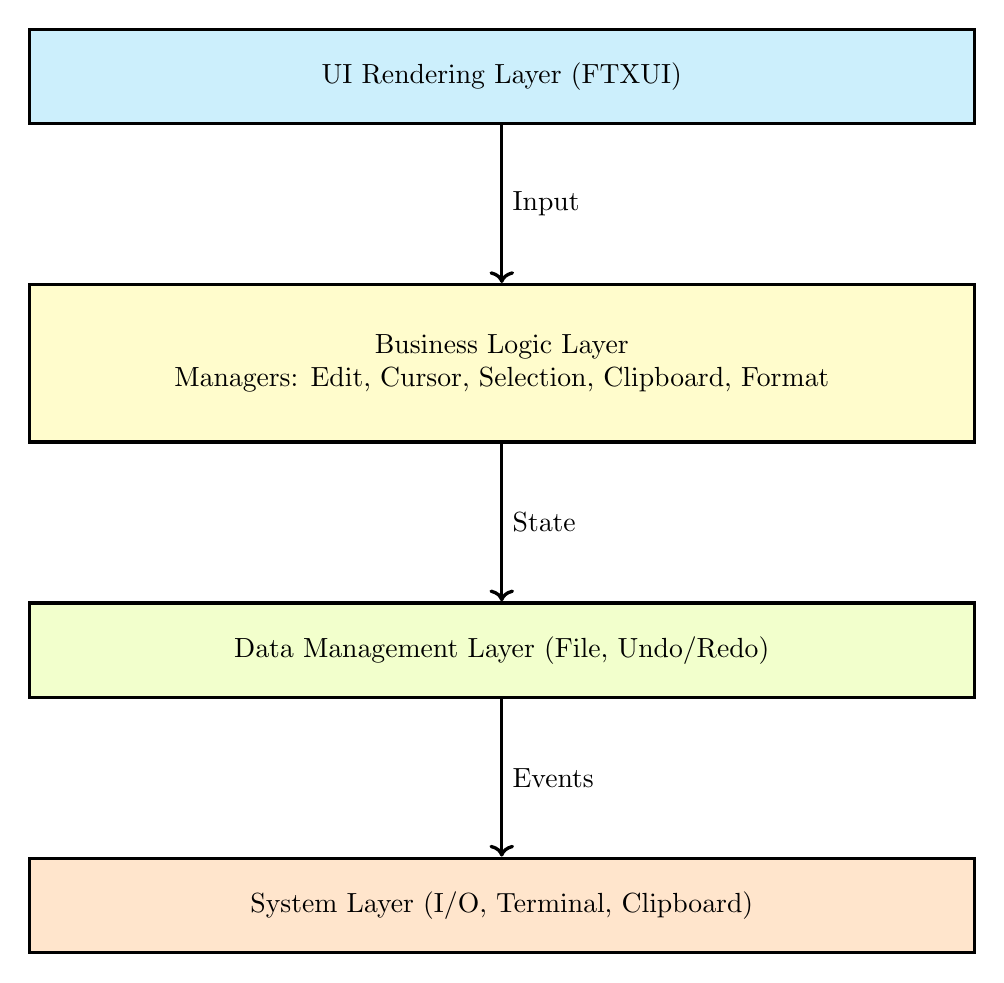
\begin{tikzpicture}[node distance=2cm]
    \node (ui) [draw, very thick, rectangle, fill=cyan!20, minimum width=12cm, minimum height=1.2cm] {UI Rendering Layer (FTXUI)};
    
    \node (business) [draw, very thick, rectangle, fill=yellow!20, minimum width=12cm, minimum height=2cm, below=of ui] {
        \begin{tabular}{c}
            Business Logic Layer \\
            Managers: Edit, Cursor, Selection, Clipboard, Format
        \end{tabular}
    };
    
    \node (data) [draw, very thick, rectangle, fill=lime!20, minimum width=12cm, minimum height=1.2cm, below=of business] {Data Management Layer (File, Undo/Redo)};
    
    \node (sys) [draw, very thick, rectangle, fill=orange!20, minimum width=12cm, minimum height=1.2cm, below=of data] {System Layer (I/O, Terminal, Clipboard)};
    
    % Arrows with labels
    \draw[->,very thick] (ui) -- node[right] {Input} (business);
    \draw[->,very thick] (business) -- node[right] {State} (data);
    \draw[->,very thick] (data) -- node[right] {Events} (sys);
\end{tikzpicture}
\caption{BZ-Nota System Architecture}
\label{fig:architecture}
\end{figure}

\section{Component Overview}

The BZ-Nota application consists of the following core components:

\begin{table}[H]
\centering
\begin{tabular}{|p{3cm}|p{8cm}|}
\hline
\textbf{Component} & \textbf{Description} \\
\hline
\textbf{Editor} & Central orchestrator managing the editing session and component coordination \\
\hline
\textbf{UI Renderer} & Renders the user interface using FTXUI framework with btop-style dashboard \\
\hline
\textbf{UI Button} & Implements dirty flag pattern for efficient button rendering \\
\hline
\textbf{Input Manager} & Handles user input events and key bindings \\
\hline
\textbf{Cursor Manager} & Manages cursor position and movement logic \\
\hline
\textbf{Selection Manager} & Handles text selection and highlighting \\
\hline
\textbf{Editing Manager} & Manages text insertion, deletion, and modification \\
\hline
\textbf{Clipboard Manager} & Manages copy/paste operations and system clipboard integration \\
\hline
\textbf{Format Manager} & Handles text formatting and Markdown marker management \\
\hline
\textbf{Formatter} & Parses and manages formatting regions with precise marker positioning \\
\hline
\textbf{File Manager} & Handles file I/O operations and file state management \\
\hline
\textbf{Undo/Redo Manager} & Implements undo/redo functionality with command pattern \\
\hline
\textbf{UTF8 Utils} & Provides UTF-8 string utilities for text processing \\
\hline
\textbf{Shared Types} & Common enums and data structures (StatusBarType, EditorMode, etc.) \\
\hline
\end{tabular}
\end{table}

% ============================================================================
% CHAPTER 3: DETAILED COMPONENT DESIGN
% ============================================================================
\chapter{Detailed Component Design}

\section{Editor Component}

\subsection{Responsibility}

The Editor component serves as the main orchestrator and controller of the application. It:

\begin{itemize}
    \item Owns and initializes all manager components
    \item Maintains the text buffer and editor state
    \item Coordinates interaction between components
    \item Manages the main event loop via FTXUI
    \item Delegates to appropriate managers based on user actions
    \item Handles application lifecycle and cleanup
\end{itemize}

\subsection{Class Structure}

\begin{lstlisting}
class Editor {
private:
    // Text buffer - each line is stored as a separate string
    std::vector<std::string> buffer;
    
    // Editor state
    bool modified = false;                              // Has unsaved changes
    int cursor_x = 0, cursor_y = 0;                    // Cursor position
    int scroll_y = 0;                                  // Viewport offset
    EditorMode editor_mode = EditorMode::FANCY;       // Current editor mode
    std::string status_message = "";
    StatusBarType status_bar_type = StatusBarType::NORMAL;
    bool debug_mode = false;                           // Debug key display mode
    
    // Manager instances (RAII - automatic construction/destruction)
    UIRenderer ui_renderer;
    SelectionManager selection_manager;
    ClipboardManager clipboard_manager;
    EditingManager editing_manager;
    CursorManager cursor_manager;
    UndoRedoManager undo_redo_manager;
    FormatManager format_manager;
    FileManager file_manager;
    InputManager input_manager;
    
public:
    Editor(const std::string& filename, bool debug_mode = false);
    ~Editor();
    void run();
    bool handle_event(ftxui::Event event);
    void render();
};
\end{lstlisting}

\section{UI Renderer Component}

\subsection{Responsibility}

The UI Renderer component is responsible for:

\begin{itemize}
    \item Converting editor state to visual output
    \item Managing terminal dimensions and layout
    \item Rendering the text buffer with syntax highlighting
    \item Displaying status bar and UI elements
    \item Handling window resizing events
\end{itemize}

\subsection{Design Details}

\begin{itemize}
    \item Built on FTXUI library for TUI rendering
    \item Implements a retained-mode rendering system
    \item Supports color output and text styling
    \item Handles VT100 escape sequences for terminal control
    \item Parses and renders Markdown formatting (bold, italic, underline, strikethrough)
    \item Supports emoji display in terminal (with fallback detection)
    \item Renders multi-pane layout (header, content, status bar, shortcuts bar)
\end{itemize}

\section{Input Manager Component}

\subsection{Responsibility}

The Input Manager handles:

\begin{itemize}
    \item Reading keyboard input from terminal
    \item Mapping key bindings to editor actions
    \item Managing input event queues
    \item Supporting special keys (arrows, function keys, etc.)
\end{itemize}

\subsection{Key Binding System}

\begin{lstlisting}
// File operations
Ctrl+S         => Save file
Ctrl+Q         => Quit (prompts if unsaved changes)
F2             => Rename file (interactive)

// Editing operations
Ctrl+Z         => Undo
Ctrl+Y         => Redo
Ctrl+A         => Select all
Ctrl+C         => Copy to system clipboard
Ctrl+X         => Cut to system clipboard
Ctrl+V         => Paste from system clipboard
Ctrl+Insert / Shift+Insert   => Traditional clipboard shortcuts
Ctrl+Shift+C / Ctrl+Shift+V  => Modern terminal clipboard
Tab            => Insert tab
Shift+Tab      => Remove leading tab (unindent)

// Formatting (Alt + key in FANCY/DOCUMENT modes)
Alt+B          => Toggle bold
Alt+I          => Toggle italic
Alt+U          => Toggle underline
Alt+T          => Toggle strikethrough

// Navigation
Arrow Keys     => Move cursor
Shift+Arrow    => Select text while moving
Ctrl+Arrow     => Jump by word
Ctrl+Shift+Arrow => Select by word (Alacritty)
Alt+Shift+Arrow  => Select by word (alternative)
Home           => Jump to start of line (smart: toggles)
End            => Jump to end of line

// Line operations
Ctrl+O         => Insert blank line above
Ctrl+K         => Insert blank line below
\end{lstlisting}

\section{Cursor Manager Component}

\subsection{Responsibility}

The Cursor Manager handles:

\begin{itemize}
    \item Cursor movement logic (up, down, left, right)
    \item Word-based movement (Ctrl+Left, Ctrl+Right)
    \item Line start/end navigation
    \item Bounds checking against buffer constraints
    \item Selection update callbacks during movement
    \item Cursor position persistence across operations
\end{itemize}

\subsection{Cursor Movement}

\begin{lstlisting}
class CursorManager {
public:
    void move_left(const std::vector<std::string>& buffer,
                   int& cursor_x, int& cursor_y,
                   CursorSelectionCallbacks callbacks, bool select);
    
    void move_right(const std::vector<std::string>& buffer,
                    int& cursor_x, int& cursor_y,
                    CursorSelectionCallbacks callbacks, bool select);
    
    void move_up(const std::vector<std::string>& buffer,
                 int& cursor_x, int& cursor_y,
                 CursorSelectionCallbacks callbacks, bool select);
    
    void move_down(const std::vector<std::string>& buffer,
                   int& cursor_x, int& cursor_y,
                   CursorSelectionCallbacks callbacks, bool select);
    
    void move_word_left(const std::vector<std::string>& buffer,
                        int& cursor_x, int cursor_y,
                        CursorSelectionCallbacks callbacks, bool select);
    
    void move_word_right(const std::vector<std::string>& buffer,
                         int& cursor_x, int cursor_y,
                         CursorSelectionCallbacks callbacks, bool select);
};
\end{lstlisting}

\section{Editor Modes}

BZ-Nota supports multiple editing modes to suit different use cases:

\subsection{BASIC Mode}

Plain text editing with no formatting support. Markdown markers like \texttt{**text**} are displayed literally without formatting applied. Suitable for code editing where you want exact byte-for-byte content.

\subsection{FANCY Mode (Default)}

Document editing with Markdown formatting support. Text wrapped in \texttt{**bold**}, \texttt{*italic*}, \texttt{<u>underline</u>}, and \texttt{\textasciitilde\textasciitilde strikethrough\textasciitilde\textasciitilde} markers is rendered with appropriate styling in the editor UI. Users can toggle formatting with Alt+B/I/U/T while typing or apply it to selections. Multiple formats can be applied on top of each other. This is the default mode suitable for note-taking and documentation.

\subsection{CODE Mode}

Syntax highlighting for programming languages with color-coded display of keywords, strings, comments, and other language constructs. No Markdown formatting rendering. Currently in development.

\subsection{DOCUMENT Mode}

Enhanced FANCY mode with planned support for dictionary checking, grammar suggestions, and document-specific features. Currently in development.

\section{Selection Manager Component}

\subsection{Responsibility}

Manages text selection with:

\begin{itemize}
    \item Selection start and end tracking
    \item Highlight rendering
    \item Selection validity maintenance
    \item Support for multiple selection modes
\end{itemize}

\subsection{Selection Modes}

\begin{enumerate}
    \item \textbf{Character Mode}: Individual character selection
    \item \textbf{Line Mode}: Full line selection
\end{enumerate}

\section{Editing Manager Component}

\subsection{Responsibility}

Core text editing operations:

\begin{itemize}
    \item Character insertion at cursor
    \item Character deletion (forward and backward)
    \item Line operations (insert, delete, split)
    \item Bulk text modifications
\end{itemize}

\subsection{Operations}

\begin{lstlisting}
class EditingManager {
public:
    void InsertCharacter(char c);
    void DeleteCharacter(bool forward = true);
    void InsertLine();
    void DeleteLine();
    void ReplaceText(const std::string& old_text, 
                    const std::string& new_text);
    void Indent(int spaces = 4);
    void Unindent(int spaces = 4);
};
\end{lstlisting}

\section{Clipboard Manager Component}

\subsection{Responsibility}

\begin{itemize}
    \item Copy selected text to system clipboard
    \item Paste from system clipboard
    \item Maintain internal clipboard buffer
    \item Handle clipboard format conversions
\end{itemize}

\section{Format Manager Component}

\subsection{Responsibility}

\begin{itemize}
    \item Manages text formatting state (bold, italic, underline, strikethrough)
    \item Wraps selected text with Markdown formatting markers
    \item Tracks active formatting modes during text input
    \item Extracts formatting metadata from selected text
    \item Handles formatting marker positioning for cursor movement
\end{itemize}

\subsection{Supported Formatting}

\begin{itemize}
    \item \textbf{Bold}: \texttt{**text**}
    \item \textit{Italic}: \texttt{*text*}
    \item \underline{Underline}: \texttt{<u>text</u>}
    \item \textbf{Strikethrough}: \texttt{~~text~~}
\end{itemize}

\subsection{Integration with EditingManager}

When text is typed with active formatting, the EditingManager automatically wraps the text with appropriate markers. When formatted text is deleted or selected, markers are preserved or removed intelligently.

\section{File Manager Component}

\subsection{Responsibility}

\begin{itemize}
    \item File I/O operations (load, save)
    \item File encoding detection and handling
    \item Error reporting with detailed messages
    \item File rename operations
    \item Path validation and security checks
\end{itemize}

\subsection{File Operations}

\begin{lstlisting}
struct FileOperationResult {
    bool success;
    std::string message;           // Human-readable message
    int error_code;                // System error code if applicable
    StatusBarType status_type;     // UI status bar type
};

class FileManager {
public:
    FileOperationResult load_file(const std::string& filename,
                                  std::vector<std::string>& buffer);
    FileOperationResult save_file(const std::string& filename,
                                  const std::vector<std::string>& buffer);
    FileOperationResult rename_file(const std::string& old_filename,
                                    const std::string& new_filename);
};
\end{lstlisting}

\section{Undo/Redo Manager Component}

\subsection{Responsibility}

Implements undo/redo with a memory-efficient diff-based approach:

\begin{itemize}
    \item Maintains undo and redo stacks of EditCommand objects
    \item Tracks line-range changes instead of full buffer snapshots
    \item Preserves cursor position before and after edits
    \item Groups related edits (typing sequences, multi-line operations)
    \item Minimizes memory usage through differential storage
\end{itemize}

\subsection{Diff-Based Command Pattern}

\begin{lstlisting}
struct EditCommand {
    int start_line;                        // First affected line
    std::vector<std::string> old_lines;   // Lines before edit
    std::vector<std::string> new_lines;   // Lines after edit
    int cursor_x_before, cursor_y_before; // Cursor position before
    int cursor_x_after, cursor_y_after;   // Cursor position after
};

class UndoRedoManager {
private:
    std::stack<EditCommand> undo_stack;
    std::stack<EditCommand> redo_stack;
    std::vector<std::string> pending_buffer; // Pending snapshot
    bool has_pending = false;
    
public:
    void save_state(const std::vector<std::string>& buffer,
                    int cursor_x, int cursor_y);
    bool undo(std::vector<std::string>& buffer,
              int& cursor_x, int& cursor_y);
    bool redo(std::vector<std::string>& buffer,
              int& cursor_x, int& cursor_y);
};
\end{lstlisting}

% ============================================================================
% CHAPTER 4: DATA STRUCTURES & SHARED TYPES
% ============================================================================
\chapter{Data Structures and Shared Types}

\section{Document Model}

The document is represented as a vector of strings:

\begin{lstlisting}
using Document = std::vector<std::string>;
\end{lstlisting}

\subsection{Advantages}

\begin{itemize}
    \item Simple to understand and implement
    \item Efficient for common operations (line-based)
    \item Easy to serialize for file I/O
    \item Natural support for line-based editing operations
    \item Efficiently integrates with undo/redo diff system
\end{itemize}

\subsection{Design Notes}

Each string in the vector represents one line of the document (without newline characters). The line count is simply the vector size. By storing lines separately rather than one continuous string, line-based operations (insertion, deletion, wrapping) are more efficient.

\section{Cursor Position}

\begin{lstlisting}
struct Position {
    int line;
    int column;
    
    bool operator==(const Position& other) const;
    bool operator<(const Position& other) const;
};
\end{lstlisting}

\section{Selection State}

\begin{lstlisting}
class SelectionManager {
private:
    bool has_selection = false;
    int selection_start_x = 0, selection_start_y = 0;
    int selection_end_x = 0, selection_end_y = 0;
    
public:
    void start_selection(int cursor_x, int cursor_y);
    void update_selection(int cursor_x, int cursor_y);
    void clear_selection();
    void select_all(int end_x, int end_y);
    
    bool has_active_selection() const;
    bool is_char_selected(int x, int y) const;
    std::string get_selected_text(const std::vector<std::string>& buffer) const;
};
\end{lstlisting}

\section{Shared Types Header}

The \texttt{shared\_types.hpp} file defines common enums and structures:

\begin{itemize}
    \item \textbf{StatusBarType}: NORMAL, SUCCESS, ERROR, WARNING
    \item \textbf{EditorAction}: Tracks last action (TYPING, DELETE, NEWLINE, etc.) for undo grouping
    \item \textbf{EditorMode}: BASIC, FANCY (with formatting), CODE (syntax highlighting), DOCUMENT (grammar features)
    \item \textbf{FormatType}: BOLD, ITALIC, UNDERLINE, STRIKETHROUGH
    \item \textbf{RenderParams}: Complete parameter bundle for UI rendering
    \item \textbf{FileOperationResult}: Result of file I/O operations with success flag and message
\end{itemize}

% ============================================================================
% CHAPTER 5: DATA FLOW AND COMPONENT INTERACTION
% ============================================================================
\chapter{Data Flow and Component Interaction}

\section{Main Event Loop}

\begin{figure}[H]
\centering
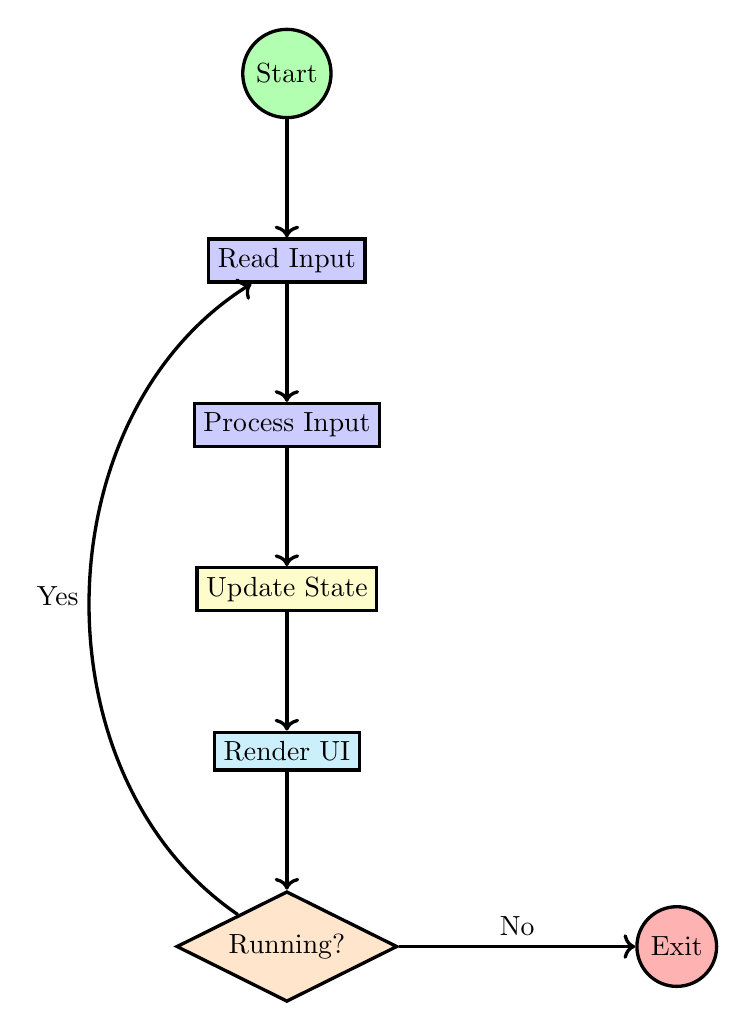
\begin{tikzpicture}[node distance=1.5cm, auto]
    \node (start) [draw, very thick, circle, fill=green!30] {Start};
    \node (input) [draw, very thick, rectangle, fill=blue!20, below=of start] {Read Input};
    \node (process) [draw, very thick, rectangle, fill=blue!20, below=of input] {Process Input};
    \node (update) [draw, very thick, rectangle, fill=yellow!20, below=of process] {Update State};
    \node (render) [draw, very thick, rectangle, fill=cyan!20, below=of update] {Render UI};
    \node (check) [draw, very thick, diamond, fill=orange!20, below=of render, aspect=2] {Running?};
    \node (end) [draw, very thick, circle, fill=red!30, right=3cm of check] {Exit};
    
    \draw[->, very thick] (start) -- (input);
    \draw[->, very thick] (input) -- (process);
    \draw[->, very thick] (process) -- (update);
    \draw[->, very thick] (update) -- (render);
    \draw[->, very thick] (render) -- (check);
    \draw[->, very thick] (check) -- node [above] {No} (end);
    \draw[->, very thick, bend left=2cm] (check) to node [left] {Yes} (input);
\end{tikzpicture}
\caption{Main Event Loop}
\label{fig:eventloop}
\end{figure}
\clearpage

\vspace*{0.5cm}
\section{Input Processing Flow}

\begin{enumerate}
    \item FTXUI reads keyboard/mouse event
    \item InputManager receives event in handle\_event()
    \item Routes to appropriate handler (ctrl keys, navigation, text input, etc.)
    \item Handler calls Editor methods or manager operations
    \item Manager updates buffer and cursor position
    \item Changes are saved to undo stack if appropriate
    \item Next render cycle shows updated content
    \item If selection is active, selection state is maintained
\end{enumerate}

\vspace{2cm}
\section{Edit Operation Flow}

\begin{table}[H]
\centering
\begin{tabular}{|l|l|l|}
\hline
\textbf{Step} & \textbf{Component} & \textbf{Action} \\
\hline
1 & Input Manager & Detect character input \\
\hline
2 & Editor & Route to Editing Manager \\
\hline
3 & Editing Manager & Insert character at cursor \\
\hline
4 & Undo/Redo Manager & Record command \\
\hline
5 & File Manager & Mark document as modified \\
\hline
6 & Format Manager & Update syntax highlighting \\
\hline
7 & UI Renderer & Re-render affected lines \\
\hline
8 & Display & Show updated content \\
\hline
\end{tabular}
\end{table}

% ============================================================================
% CHAPTER 6: DESIGN PATTERNS
% ============================================================================
\chapter{Design Patterns and Principles}

\section{Used Design Patterns}

\subsection{Model-View-Controller (MVC)}

\begin{itemize}
    \item \textbf{Model}: Document and editor state
    \item \textbf{View}: UI Renderer
    \item \textbf{Controller}: Input Manager and Editor
\end{itemize}

\subsection{Command Pattern}

Implemented in the Undo/Redo Manager for:

\begin{itemize}
    \item Encapsulating requests as objects
    \item Enabling undo/redo functionality
    \item Supporting command queuing
    \item Logging and auditing changes
\end{itemize}

\subsection{Observer Pattern}

For:

\begin{itemize}
    \item Notifying components of document changes
    \item UI update triggers
    \item Event-driven architecture
\end{itemize}

\subsection{Singleton Pattern}

Not actively used in current implementation.

\subsection{Factory Pattern}

For:

\begin{itemize}
    \item Creating Command objects
    \item Instantiating formatters for file types
\end{itemize}

\section{SOLID Principles}

\subsection{Single Responsibility Principle}

Each component has one clear responsibility:

\begin{itemize}
    \item Cursor Manager: Cursor operations
    \item File Manager: File I/O
    \item Editing Manager: Text modification
\end{itemize}

\subsection{Open/Closed Principle}

\begin{itemize}
    \item Open for extension via inheritance
    \item Closed for modification of stable interfaces
\end{itemize}

\subsection{Liskov Substitution Principle}

\begin{itemize}
    \item Command subclasses are properly substitutable
    \item Formatter implementations follow contracts
\end{itemize}

\subsection{Interface Segregation Principle}

\begin{itemize}
    \item Components expose only necessary operations
    \item Minimal coupling between components
\end{itemize}

\subsection{Dependency Inversion Principle}

\begin{itemize}
    \item Editor depends on abstractions
    \item Manager interfaces are stable
\end{itemize}

% ============================================================================
% CHAPTER 7: TECHNOLOGY STACK
% ============================================================================
\chapter{Technology Stack}

\section{Core Technologies}

\begin{table}[H]
\centering
\begin{tabular}{|l|l|l|}
\hline
\textbf{Component} & \textbf{Technology} & \textbf{Purpose} \\
\hline
Language & C++17 & High performance, modern features \\
\hline
Build System & CMake 3.10+ & Cross-platform build automation \\
\hline
UI Framework & FTXUI & Terminal UI rendering \\
\hline
Platform & Linux/Unix & Target deployment platform \\
\hline
\end{tabular}
\end{table}

\section{FTXUI Framework}

FTXUI is a C++ library for building TUI applications.

\subsection{Why FTXUI?}

\begin{itemize}
    \item Cross-platform TUI rendering
    \item Component-based architecture
    \item Rich color and styling support
    \item Active community and maintenance
    \item Lightweight and performant
\end{itemize}

\subsection{Key Features}

\begin{itemize}
    \item Reactive component model
    \item Canvas and text rendering
    \item Event handling system
    \item Unicode and UTF-8 support
    \item Color palette management
\end{itemize}

% ============================================================================
% CHAPTER 8: ERROR HANDLING & LOGGING
% ============================================================================
\chapter{Error Handling and Logging}

\section{Error Handling Strategy}

\subsection{Exception Hierarchy}

\begin{lstlisting}
class EditorException : public std::exception {
public:
    explicit EditorException(const std::string& msg);
    const char* what() const noexcept override;
private:
    std::string message_;
};

class FileException : public EditorException {};
class EditingException : public EditorException {};
class ClipboardException : public EditorException {};
\end{lstlisting}

\subsection{Error Categories}

\begin{table}[H]
\centering
\begin{tabular}{|l|p{6cm}|}
\hline
\textbf{Category} & \textbf{Examples} \\
\hline
File Errors & File not found, permission denied, I/O errors \\
\hline
Input Errors & Invalid cursor position, boundary violations \\
\hline
System Errors & Clipboard unavailable, terminal errors \\
\hline
Resource Errors & Memory allocation failures \\
\hline
\end{tabular}
\end{table}

\section{Logging System}

\subsection{Log Levels}

\begin{enumerate}
    \item \textbf{DEBUG}: Detailed diagnostic information
    \item \textbf{INFO}: General information messages
    \item \textbf{WARNING}: Recoverable issues
    \item \textbf{ERROR}: Failures
    \item \textbf{FATAL}: Application exit required
\end{enumerate}

\subsection{Implementation}

\begin{itemize}
    \item Singleton logger instance
    \item File and console output support
    \item Timestamp and severity level tracking
    \item Thread-safe logging operations
\end{itemize}

% ============================================================================
% CHAPTER 9: PERFORMANCE CONSIDERATIONS
% ============================================================================
\chapter{Performance Considerations}

\section{Optimization Strategies}

\subsection{Rendering Optimization}

\begin{itemize}
    \item Dirty region tracking for selective redraws
    \item Buffer caching for unchanged content
    \item Minimal terminal escape sequence output
    \item Viewport-based rendering
\end{itemize}

\subsection{Memory Management}

\begin{itemize}
    \item Efficient string storage
    \item Smart pointers for automatic cleanup
    \item Pre-allocated buffers
    \item Move semantics to avoid copies
\end{itemize}

\subsection{Input Processing}

\begin{itemize}
    \item Non-blocking input reading
    \item Input event batching
    \item Efficient key binding lookup
\end{itemize}

\section{Benchmarking Targets}

\begin{table}[H]
\centering
\begin{tabular}{|l|c|}
\hline
\textbf{Operation} & \textbf{Target Time} \\
\hline
Character insertion & $< 1$ ms \\
\hline
Line deletion & $< 5$ ms \\
\hline
File open (1MB) & $< 100$ ms \\
\hline
Screen refresh & $< 16$ ms (60 FPS) \\
\hline
\end{tabular}
\end{table}

% ============================================================================
% CHAPTER 10: SECURITY CONSIDERATIONS
% ============================================================================
\chapter{Security Considerations}

\section{Input Validation}

\begin{itemize}
    \item Validate all file inputs
    \item Sanitize keyboard input
    \item Boundary checking on array accesses
    \item Check file permissions
\end{itemize}

\section{File Operations}

\begin{itemize}
    \item Secure file creation with proper permissions
    \item Validate file paths (prevent directory traversal)
    \item Atomic file writing (write-then-rename)
    \item Backup original before in-place modification
\end{itemize}

\section{Buffer Security}

\begin{itemize}
    \item Use standard containers (std::string, std::vector)
    \item Avoid manual buffer management
    \item Enable compiler security flags
    \item Use AddressSanitizer for development
\end{itemize}

% ============================================================================
% CHAPTER 11: TESTING STRATEGY
% ============================================================================
\chapter{Testing Strategy}

\section{Test Categories}

\subsection{Unit Testing}

\begin{itemize}
    \item Cursor position calculations
    \item Text editing operations
    \item File I/O operations
    \item Selection logic
\end{itemize}

\subsection{Integration Testing}

\begin{itemize}
    \item Edit operation with undo/redo
    \item File open/edit/save cycle
    \item Copy/paste operations
\end{itemize}

\subsection{System Testing}

\begin{itemize}
    \item Full editing sessions
    \item Different file types and encodings
    \item Large file handling
    \item Terminal size variations
\end{itemize}

\subsection{Performance Testing}

\begin{itemize}
    \item Benchmark common operations
    \item Large file editing performance
    \item Memory usage profiling
    %\item Rendering frame rate measurement
\end{itemize}

% ============================================================================
% CHAPTER 12: BUILD & DEPLOYMENT
% ============================================================================
\chapter{Build and Deployment}

\section{Build System}

CMake 3.10+ is the primary build system with support for:

\begin{itemize}
    \item Multiple compiler support (GCC, Clang)
    \item Release and Debug configurations
    \item Static and dynamic linking
    \item Cross-compilation support
\end{itemize}

\subsection{Build Targets}

\begin{table}[H]
\centering
\begin{tabular}{|l|p{6cm}|}
\hline
\textbf{Target} & \textbf{Description} \\
\hline
bznota & Main executable \\
\hline
bznota-tests & Unit test executable \\
\hline
bznota-install & Installation target \\
\hline
\end{tabular}
\end{table}

\section{Compilation}

\subsection{CMake Configuration}

\begin{lstlisting}
mkdir build && cd build
cmake ..
cmake --build .
\end{lstlisting}

\section{Installation}

\begin{lstlisting}
sudo cmake --install . --prefix /usr/local
\end{lstlisting}

\subsection{Install Structure}

\begin{itemize}
    \item Binary: \texttt{/usr/local/bin/bznota}
    \item Man page: \texttt{/usr/local/share/man/man1/bznota.1}
    \item Desktop entry: \texttt{/usr/share/applications/bznota.desktop}
\end{itemize}

% ============================================================================
% CHAPTER 13: CONTRIBUTING GUIDELINES
% ============================================================================
\chapter{Contributing Guidelines and Project Maintenance}

\section{Code Style}

\subsection{Naming Conventions}

\begin{itemize}
    \item Classes: \texttt{PascalCase} (e.g., \texttt{CursorManager}, \texttt{EditingManager})
    \item Methods: \texttt{snake\_case} (e.g., \texttt{move\_left()}, \texttt{insert\_char()})
    \item Constants: \texttt{UPPER\_SNAKE\_CASE} (e.g., \texttt{MAX\_BUFFER\_SIZE})
    \item Member variables: \texttt{snake\_case} with trailing underscore (legacy) or no underscore (current)
    \item Function parameters: \texttt{snake\_case}
\end{itemize}

\subsection{Code Formatting}

\begin{itemize}
    \item Use 4 spaces for indentation
    \item Max line length: 100 characters
    \item Use clang-format for auto-formatting
    \item K\&R style brace placement
\end{itemize}

\section{Documentation Standards}

\begin{itemize}
    \item Doxygen comments for public interfaces
    \item Include usage examples
    \item Update TDD for architectural changes
    \item Keep README in sync with features
\end{itemize}

\section{Git Workflow}

\begin{itemize}
    \item Feature branches: \texttt{feature/feature-name}
    \item Bugfix branches: \texttt{bugfix/bug-name}
    \item Semantic commit messages
    \item Pull request reviews required
\end{itemize}

% ============================================================================
% CHAPTER 14: APPENDICES
% ============================================================================
\chapter*{Appendices}
\addcontentsline{toc}{chapter}{Appendices}

\section*{A. File Structure Reference}

\begin{table}[H]
\centering
\begin{tabular}{|l|p{8cm}|}
\hline
\textbf{File} & \textbf{Purpose} \\
\hline
editor.hpp/cpp & Main editor and event loop orchestrator \\
\hline
ui\_renderer.hpp/cpp & FTXUI rendering engine; parses markdown formatting; implements btop-style dashboard \\
\hline
ui\_button.hpp/cpp & Implements dirty flag pattern for efficient button rendering \\
\hline
input\_manager.hpp/cpp & Keyboard/mouse event handling and key binding dispatch \\
\hline
cursor\_manager.hpp/cpp & Cursor movement logic and boundary checking \\
\hline
selection\_manager.hpp/cpp & Text selection state and selection-aware operations \\
\hline
editing\_manager.hpp/cpp & Text insertion/deletion and buffer modifications \\
\hline
clipboard\_manager.hpp/cpp & System clipboard integration (X11/Wayland) \\
\hline
format\_manager.hpp/cpp & Text formatting state and markdown marker management \\
\hline
formatter.hpp/cpp & Parses and manages formatting regions with precise marker positioning \\
\hline
file\_manager.hpp/cpp & File I/O operations and error handling \\
\hline
undo\_redo\_manager.hpp/cpp & Diff-based undo/redo with EditCommand history \\
\hline
shared\_types.hpp & Common enums and data structures (StatusBarType, EditorMode, etc.) \\
\hline
utf8\_utils.hpp/cpp & UTF-8 string utilities for text processing \\
\hline
version.hpp.in & Version number template (filled by CMake) \\
\hline
\end{tabular}
\end{table}

\section*{B. Component Dependency Graph}

\begin{figure}[H]
\centering
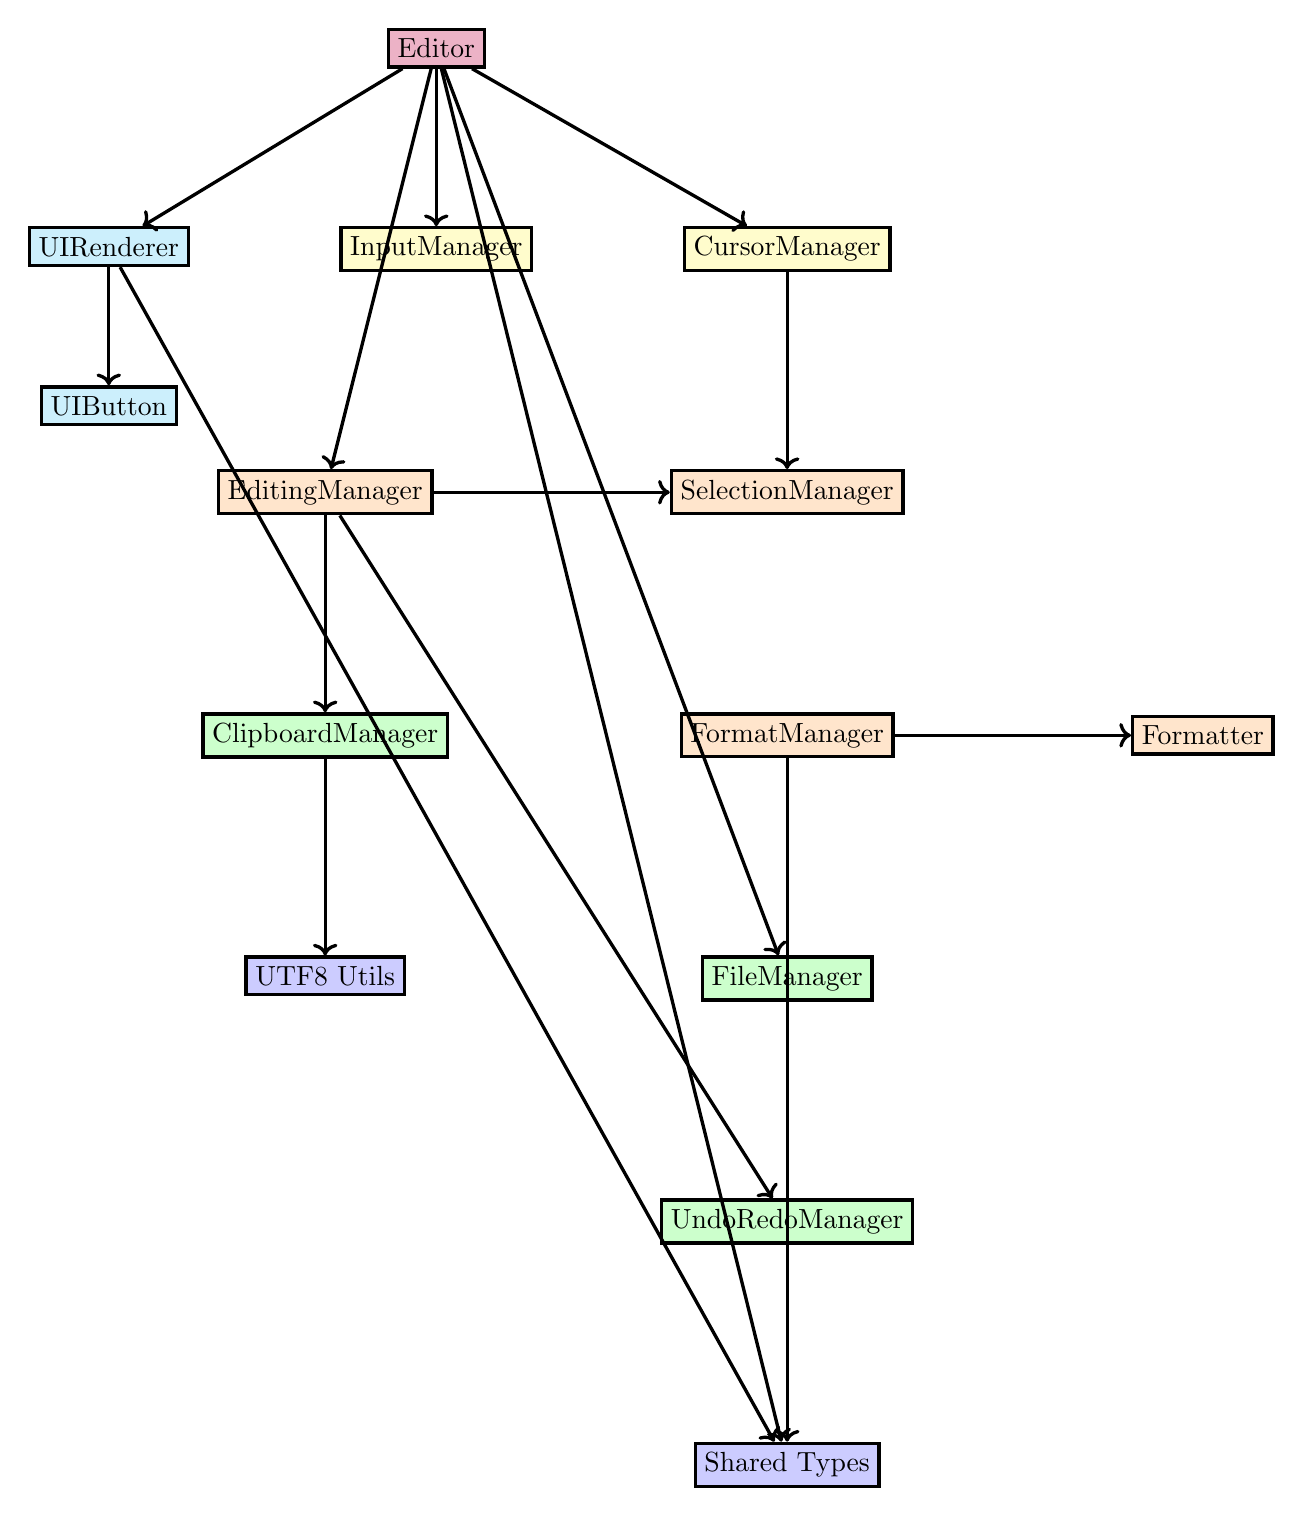
\begin{tikzpicture}[->, very thick, node distance=2.2cm]
    \node (editor) [draw, very thick, rectangle, fill=purple!30] {Editor};
    \node (ui) [draw, rectangle, fill=cyan!20, below left=2cm and 2.5cm of editor] {UIRenderer};
    \node (ui_button) [draw, rectangle, fill=cyan!20, below=1.5cm of ui] {UIButton};
    \node (input) [draw, rectangle, fill=yellow!20, below=2cm of editor] {InputManager};
    \node (cursor) [draw, rectangle, fill=yellow!20, below right=2cm and 2.5cm of editor] {CursorManager};
    
    \node (selection) [draw, rectangle, fill=orange!20, below=2.5cm of cursor] {SelectionManager};
    \node (editing) [draw, rectangle, fill=orange!20, left=3cm of selection] {EditingManager};
    \node (clipboard) [draw, rectangle, fill=green!20, below=2.5cm of editing] {ClipboardManager};
    
    \node (format) [draw, rectangle, fill=orange!20, below=2.5cm of selection] {FormatManager};
    \node (formatter) [draw, rectangle, fill=orange!20, right=3cm of format] {Formatter};
    \node (file) [draw, rectangle, fill=green!20, below=2.5cm of format] {FileManager};
    \node (undo) [draw, rectangle, fill=green!20, below=2.5cm of file] {UndoRedoManager};
    \node (utf8) [draw, rectangle, fill=blue!20, below=2.5cm of clipboard] {UTF8 Utils};
    \node (shared) [draw, rectangle, fill=blue!20, below=2.5cm of undo] {Shared Types};
    
    \draw (editor) -- (ui);
    \draw (ui) -- (ui_button);
    \draw (editor) -- (input);
    \draw (editor) -- (cursor);
    \draw (editor) -- (editing);
    \draw (editor) -- (file);
    \draw (editing) -- (undo);
    \draw (editing) -- (clipboard);
    \draw (editing) -- (selection);
    \draw (cursor) -- (selection);
    \draw (format) -- (formatter);
    \draw (clipboard) -- (utf8);
    \draw (editor) -- (shared);
    \draw (ui) -- (shared);
    \draw (format) -- (shared);
\end{tikzpicture}
\caption{Component Dependency Graph}
\label{fig:dependencies}
\end{figure}

\section*{C. Troubleshooting Guide}

\begin{table}[H]
\centering
\begin{tabular}{|p{4cm}|p{7cm}|}
\hline
\textbf{Issue} & \textbf{Solution} \\
\hline
FTXUI compilation error & Update FTXUI submodule: \texttt{git submodule update --recursive} \\
\hline
Terminal size issues & SIGWINCH handler automatically manages resize events \\
\hline
Clipboard not working & Verify xclip/wl-copy installed; check \$DISPLAY or Wayland setup \\
\hline
Formatting not displaying & Ensure editor mode is FANCY or DOCUMENT (not BASIC or CODE) \\
\hline
Button rendering issues & Check UIButton dirty flag implementation; verify FTXUI element caching \\
\hline
Markdown parsing errors & Verify formatter.hpp/cpp implementation; check marker positioning logic \\
\hline
UTF-8 text display problems & Check utf8\_utils.hpp/cpp for proper encoding handling \\
\hline
High latency & Profile input event handling; check for slow file operations \\
\hline
Memory leaks & Run with AddressSanitizer: \texttt{-fsanitize=address} \\
\hline
\end{tabular}
\end{table}

% ============================================================================
% CONCLUSION
% ============================================================================
\chapter*{Conclusion}
\addcontentsline{toc}{chapter}{Conclusion}

BZ-Nota is designed as a modern, performant terminal-based text editor with a modular, maintainable architecture. The separation of concerns across multiple manager components allows for independent development, testing, and extension of features.

The design follows proven software engineering principles and patterns, ensuring code quality and long-term maintainability. With its foundation on robust technologies like C++17 and FTXUI, BZ-Nota is positioned for continued growth and enhancement.

This Technical Design Document serves as the canonical reference for the system architecture and will be maintained alongside the codebase throughout the project lifecycle.

% ============================================================================
% REFERENCES
% ============================================================================
\chapter*{References}
\addcontentsline{toc}{chapter}{References}

\begin{itemize}
    \item FTXUI: \url{https://github.com/ArthurSonzogni/FTXUI}
    \item C++17 Standard: ISO/IEC 14882:2017
    \item CMake Documentation: \url{https://cmake.org/}
    \item Google C++ Style Guide: \url{https://google.github.io/styleguide/cppguide.html}
    \item Design Patterns: Gang of Four, Design Patterns: Elements of Reusable Object-Oriented Software
    \item SOLID Principles: Robert C. Martin, Clean Code
\end{itemize}

\end{document}
